\section{Experiments}

\section{Results}

\begin{table}[h]
    \centering
    \begin{tabular}{l l l l }
    \toprule
    Condition & DNN & CNN & AUG \\ \midrule
    Base & 91.45 & 94.45 &  90.56\\
    Opening & 94.58 & 99.11 &  95.10\\
    Low Pressure &  92.92 & 96.63 & 93.54\\
    \bottomrule
    \end{tabular}
    \caption{Leave one group out cross validation}
	\label{tab:baseexps}
\end{table}

\begin{table}[h]
    \centering
    \begin{tabular}{l l l l}
    \toprule
    Condition & Noise Type & DNN & CNN \\ \midrule
    Base & Workshop &  67.70 & 68.42 \\
    Opening & Workshop & 47.52 & 59.81 \\
    Low Pressure & Workshop & 65.83 & 75.21 \\ \midrule
    Base & Hydraulic  & 39.74& 33.49  \\
    Opening & Hydraulic & 45.16 & 42.84  \\
    Low Pressure & Hydraulic & 66.72 & 58.56 \\
    \bottomrule
    \end{tabular}
    \caption{Train with normal test with low noise}
	\label{tab:baseexps}
\end{table}




%%% OLD RESULTS %%%%
% \section{Results}


% [...]
% Visible in figure \ref{fig:meanfracc} 
% - mean accuracy values of all experiments per microphone position
% - arithmetic mean (black) and max deviation (grey)
% - similar mean accuracy at similar distance 
% - odd numbers (high gain) in microphone pairs have lower mean accuracy than even numbers (low gain)

% \begin{figure}[h]
% 	\centering
% 	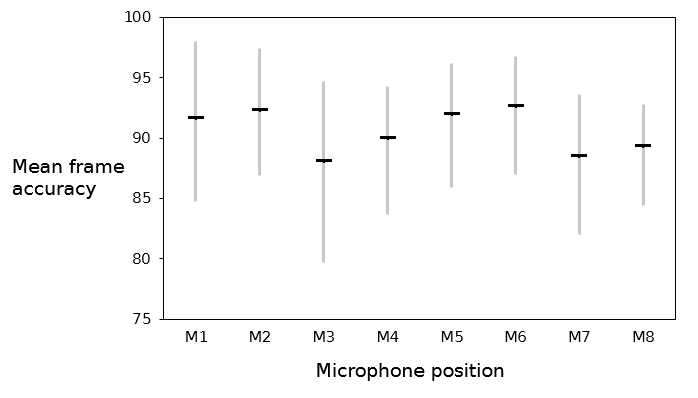
\includegraphics[width=88mm]{images/mean_frame_acc.png}
% 	\caption{Spectrogram of leakage noise from microfone position 1 with characteristic vent flow rate for 6 Bar}
% 	\label{fig:meanfracc}
% \end{figure}

% \iffalse


% \begin{figure}[h]
% 	\centering
% 	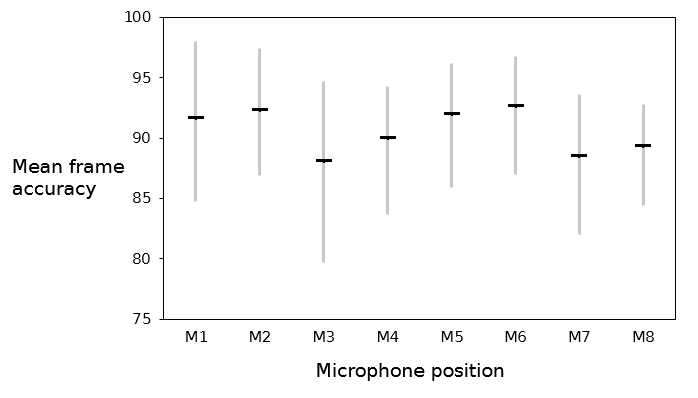
\includegraphics[width=88mm]{images/mean_frame_acc.png}
% 	\caption{Mean (frame) detection accuracy per microphone position (M)}
% 	\label{fig:mean_frame_acc}
% \end{figure}




% \begin{table}[h]
%     \centering
%     \begin{tabular}{lllllllll}
%     & 1m    & 1l    & 2m    & 2l    & 3m    & 3l    & 4m    & 4l    \\
%     \hline
%     v  & 97,97 & 96,06 & 94,65 & 94,23 & 95,19 & 94,62 & 93,22 & 91,86 \\
%     p  & 93,16 & 92,37 & 82,85 & 83,69 & 93,7  & 93,04 & 90,09 & 87    \\
%     o  & 97,81 & 97,4  & 93,65 & 93,52 & 94,83 & 96,72 & 93,63 & 88,56 \\
%     w  & 92,86 & 91,38 & 90,36 & 90,31 & 90,04 & 93,04 & 90,34 & 90,26 \\
%     h  & 92,29 & 93,69 & 88,52 & 93,51 & 96,15 & 94,88 & 89,2  & 92,55 \\
%     po & 93,54 & 93,51 & 91,76 & 90,96 & 93,18 & 94,46 & 90,52 & 92,8  \\
%     oh & 86,17 & 92,01 & 79,68 & 90,92 & 90,8  & 89,55 & 82,09 & 89,27 \\
%     ow & 86,81 & 87,86 & 85,29 & 85,4  & 87,77 & 90,61 & 85,65 & 84,37 \\
%     ph & 84,7  & 86,93 & 86,35 & 87,06 & 85,93 & 86,96 & 81,97 & 87,27 \\
%     \hline
%     \caption{Mean frame accuracy for microphone positions}
% 	\label{tab:mappingclasses}
%     \end{tabular}
% \end{table}